\chapter*{Introduction}
\label{chap:intro}
% \epigraph{\itshape  La volonté trouve, la liberté choisit. Trouver et choisir, c'est penser}{-- Victor Hugo}
% \startcontents[chapters]
\addcontentsline{toc}{chapter}{Introduction}  
\fancyhead[LE,RO]{Introduction}

\phantomsection
\addcontentsline{toc}{section}{Généralités}
\section*{Context}

\phantomsection
\addcontentsline{toc}{section}{Généralités}
\section*{Question}

\phantomsection
\addcontentsline{toc}{section}{Mon boulot à moi}
\section*{Objectives and positioning}

\phantomsection
\addcontentsline{toc}{section}{Mon boulot à moi}
\section*{M}

 \noindent Test pour le glossaire~:  \Gls{latex} et \Gls{EPISEN}. \Gls{prefixe}.
 \gls{prefixe}


 \noindent Acronyme: \glsxtrshort{gcd} et nous rappelons qu'un \glsxtrshort{gcd} est~: 

\glsxtrlong{gcd} 

 \noindent Et bien sûr \glsxtrshort{llm} mais chat-gpt n'est pas trop autorisé pour écrire les mémoires !  


\noindent Test pour la bibliographie~:
\begin{itemize}
\item Un article de revue \cite{ref1}~;
\item Deux articles de revue \cite{ref2,ref1}~;
\item Article de Conférence \cite{ref3}~;
\item Un livre \cite{ref4}
\item Une thèse \cite{ref5}
\item Tout le monde (test ordre) \cite{ref4,ref1,ref5,ref2,ref3}.
\end{itemize}

Vous trouverez un exemple de tableau de données à mettre dans ce manuscrit
mais aussi dans le poster et dans le diaporama à la Figure~\ref{fig:tab1}.

On peut aussi mettre des images (ou des figures gnuplot, voir des tutos), pour faire des figures et compléter le poster/diaporama. Cela est visible, par exemple, à la Figure~\ref{fig:logo}. 

\begin{figure}[!t]
\begin{center}
\begin{tabular}{|l|l|l|}
\hline
Département & Nombre de chaises & Nombre de prises électriques\\
\hline
\hline
ITS & 150 & 20\\
\hline
SI & 149 & 25 \\
\hline
ISBS & 151 & 19\\
\hline
\end{tabular}
\end{center}
\caption{Un exemple de tableau dans tout les supports.}
\label{fig:tab1}
\end{figure}


\begin{figure}[!t]
\begin{center}
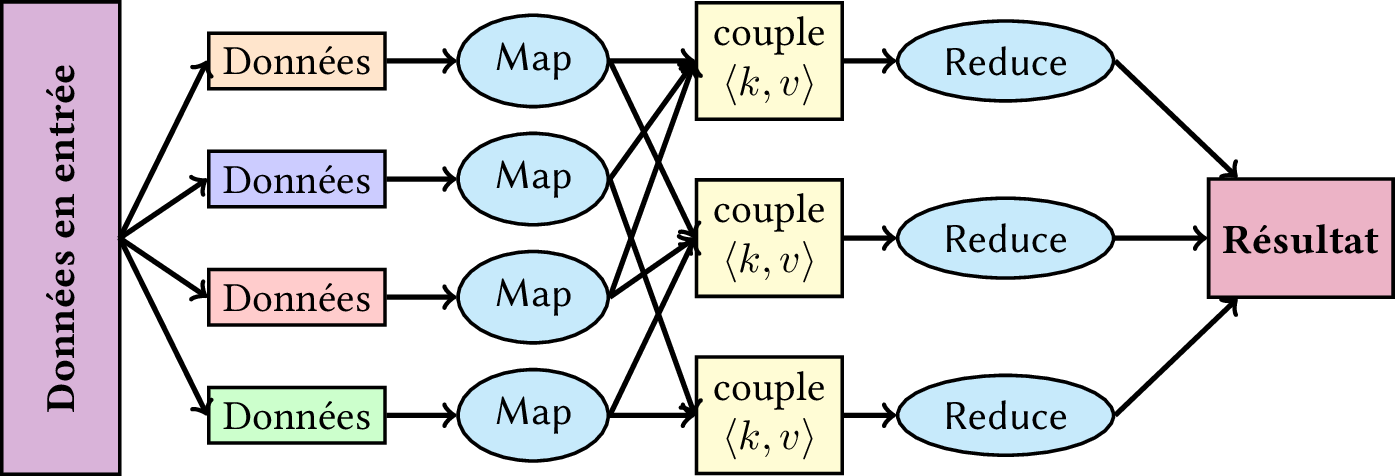
\includegraphics[height=5cm]{../images/Mapreduce.png}
\end{center}
\caption{Un exemple de figure avec dessin (png).}
\label{fig:logo}
\end{figure}

Cela est bien sûr aussi possible pour un listing de points importants que l'on souhaite voir dans ce manuscrit ainsi que dans le diaporama ou le poster. Exemple, ll est très important de~:
\begin{itemize}
	\item Citer vos sources~;
	\item Référencer les figures dans le texte~;
	\item Avoir une notation cohérente entre les différents supports~;
	\item Respecter le typographie pour le bien être du relecteur.
\end{itemize}


On peut aussi mettre faire cela pour de jolies formules mathématiques dont on peut changer le contenu dans tout les supports si cela est dans un fichier séparé. Exemple~:
\input{../ShareText/maths1.tex}

Plutôt pratique non ?

\begin{itemize}
\item \underline{souligné}
\item {\bf en gras} ou \textbf{text}
\item {\it italique} ou \textit{text}
\end{itemize}

\phantomsection
\addcontentsline{toc}{section}{Plan}
\section*{Plan}
Et on n'oublie pas le plan du mémoire à la fin de l'introduction. Exemple~:
Nous parlerons de ... au Chapitre~\ref{chap:one} avec au début dans la Section~\ref{sec:one:one} à la page \pageref{sec:one:one} puis de ... dans la Section~\ref{sec:one:two} à la page \pageref{sec:one:two}. Dans le Chapitre~\ref{chap:two} nous continuerons à analyser... notamment avec l'exemple de blibli dans la Section~\ref{sec:two:one} à la page \pageref{sec:two:one} et puis le cas particulier de blabla dans la Section~\ref{sec:two:two} à la page \pageref{sec:two:two}.


\textit{etc.}

Et nous terminerons par la Conclusion à la page \pageref{chap:conclu}.

Il est à noter que vous trouverez certains codes dans l'Annexe~\ref{annexe:one} à la page \pageref{annexe:one} et tout les données dans l'Annexe~\ref{annexe:two} à la page \pageref{annexe:two}.
